Una vez llevado a cabo el desarrollo teórico de la aplicación y los cálculos necesarios para llegar a los resultados deseados, el siguiente paso será aplicar estos a un emplazamiento concreto, observar los resultados obtenidos y analizarlos para sacar una conclusión.

Éste capítulo también servirá como una guía detallada de uso de la aplicación, explicando la información a introducir en cada paso y como obtenerlos.

La aplicación está disponible a través del enlace \url{http://solarcalc.app} para utilizarse de manera totalmente gratuita.

\section{Obtención de datos del usuario}

El formulario que se le presenta al usuario para que éste introduzca la información de su emplazamiento es el siguiente:
\begin{figure}[ht]
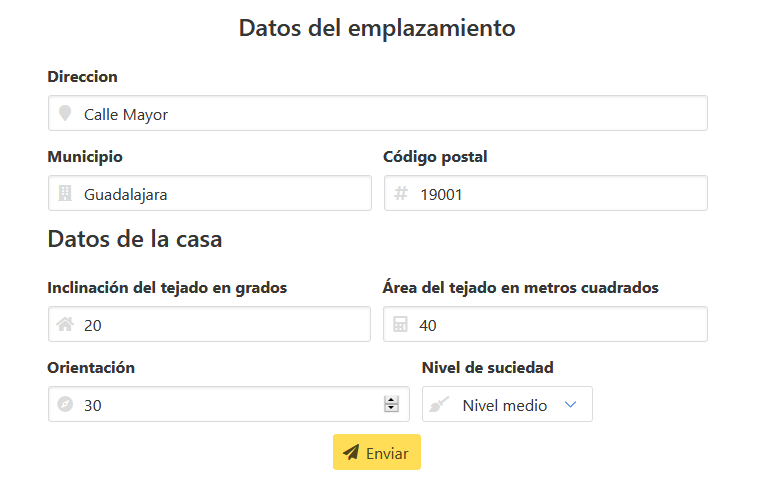
\includegraphics[scale=0.4]{USER_FORM}
\centering
\caption{Formulario web para obtención de datos}
\label{fig:user_form}
\end{figure}

Como se puede observar, el formulario consta de dos partes, por un lado está la dirección como tal, que se utilizará para obtener las coordenadas del emplazamiento y por otro está la configuración física de la superficie destinada a la instalación de los paneles solares.

\subsection{Latitud y longitud a partir de la dirección}

La primera parte del formulario consiste en obtener la información acerca del emplazamiento del usuario, es decir, su latitud y longitud. Estos datos son los que se utilizarán en el código, para obtener la información de la radiación en dicho lugar.

Para ello, el formulario pide una dirección, que no necesariamente tiene que ser la exacta del emplazamiento, sino que se puede utilizar una dirección genérica cercana al lugar donde se va a realizar la instalación, ya que para una distancia relativamente corta la radiación solar no variará de manera notable.

En este caso práctico la dirección que utilizaremos será la de Guadalajara. Para ésta dirección, las coordenadas que Google nos devuelve son:
\begin{itemize}
\item \textbf{Latitud:} $40,632 \degree$.
\item \textbf{Longitud:} $-3.166 \degree$.
\end{itemize}

\subsection{Datos de la superficie destinada a la instalación}

Una vez obtenidas las coordenadas del emplazamiento, es necesario conocer la inclinación, la orientación y el nivel de suciedad de la superficie, para poder realizar el cambio de la radiación en el plano horizontal obtenida anteriormente a la radiación eficaz incidente.

Para ello el formulario nos ofrece 4 campos de información:

\begin{itemize}
\item \textbf{Inclinación en grados:} Para obtener la inclinación de la superficie en grados se puede utilizar cualquier smartphone actual dotado con un sensor giroscópico y una aplicación de tipo nivel, algún dispositivo de medición de ángulos como un transportador.
\item \textbf{Orientación:} Para la obtener la orientación de la superficie se puede utilizar una brújula, ya sea analógica o digital. Se considera que 0 grados es el SUR.
\item \textbf{Área del tejado:} Simplemente el área que se desea cubrir con paneles solares.
\item \textbf{Nivel de suciedad:} Este campo es el mas subjetivo y será a criterio del usuario. Se recomienda realizar cálculos con el peor caso para establecer un margen pero, no obstante, si se conoce con seguridad cuál es el nivel de suciedad de la zona, se ha de usar éste.
\end{itemize}

\section {Aplicación de los datos al proceso de cálculo}

En la sección anterior hemos recogido los datos que un usuario ha introducido a través del formulario. Estos datos son:
\begin{itemize}
\item \textbf{Latitud:} $40,632 \degree$.
\item \textbf{Longitud:} $-3.166 \degree$.
\item \textbf{Inclinación de la superficie:} $20 \degree$.
\item \textbf{Área de la superficie:} $40 m^2 $.
\item \textbf{Orientación de la superficie:} $30 \degree$.
\item \textbf{Nivel de suciedad:} Medio.
\end{itemize}

A continuación, utilizaremos estos datos para recorrer numéricamente el proceso teórico descrito en el capítulo anterior. 

\subsection{Valores medios mensuales de radiación global}

Tal y como se menciona en la sección \ref{section:get_global_rad}, el primer paso para poder llevar a cabo el proceso de cálculo de la radiación incidente eficaz es obtener la radiación global media para cada uno de los doce meses, en el emplazamiento indicado por el usuario.

Para las coordenadas introducidas por el usuario, el punto con información mas cercano que tenemos es de latitud  $40,57 \degree$ y longitud $-3.16 \degree$. 

Para este punto, los valores de irradiación media son:
\begin{table}[ht]
\centering
\begin{tabular}{|l|l|l|l|l|l|l|l|l|l|l|l|l|}
\hline
$kWh/m^2$   & Ene & Feb & Mar & Abr & May & Jun & Jul & Ago & Sept & Oct & Nov & Dic \\ \hline
Valor medio & 2,0 & 3,1 & 4,8 & 5,7 & 6,8 & 8,0 & 7,8 & 6,8 & 5,1  & 3,5 & 2,2 & 1,7 \\ \hline
\end{tabular}
\label{tab:mean_values_monthly}
\caption{Irradiación global media mensual}
\end{table}

\subsection{Irradiancia extra-terrestre diaria}

Además, por otro lado, para poder continuar con el proceso de cálculo, es necesario calcular la irradiancia extra-terrestre diaria, utilizando la latitud indicada por el usuario y los días promedio de la tabla \ref{tab:dias_promedio}.
En las ecuaciones de la sección \ref{section:extra-irrad} se indican los pasos a seguir y el resultado es:
\begin{table}[ht]
\centering
\begin{tabular}{|l|l|l|l|l|l|l|l|l|l|l|l|l|}
\hline
$kW/m^2$   & Ene & Feb & Mar & Abr & May & Jun & Jul & Ago & Sept & Oct & Nov & Dic \\ \hline
$B_{0d}(0)$ & 4,12 & 5,48 & 7,47 & 9,57 & 11,01 & 11,59 & 11,26 & 10,01 & 8,05 & 5,90  & 4,30 & 3,58 \\ \hline
\end{tabular}
\label{tab:extra_irrad_values}
\caption{Irradiancia extra-terrestre diaria}
\end{table}

\subsection{Separación de la radiación global horizontal en sus componentes}

Una vez conocidos los valores mensuales de la radiación global en el plano horizontal, el siguiente paso se centra en separar la radiación global en sus dos componentes, la directa y la difusa, tal y como se explica en la sección \ref{section:radiation_components}.

Como podemos observar en la ecuación \ref{eqn:ktd}, el primer paso para separar la irradiación global en sus dos componentes es calcular el índice de claridad, para que posteriormente calculemos la fracción de radiación difusa. 
\newpage

Si aplicamos dicha ecuación a los resultados anteriores obtenemos los siguiente resultados:

\begin{table}[ht]
\centering
\begin{tabular}{|l|l|l|l|l|l|l|l|l|l|l|l|l|}
\hline
    & Ene & Feb & Mar & Abr & May & Jun & Jul & Ago & Sept & Oct & Nov & Dic \\ \hline
$K_{Td}$ & 0,485 & 0,565 & 0,642 & 0,595 & 0,617 & 0,690 & 0,692 & 0,679 & 0,632 & 0,592 & 0,511  & 0,461  \\ \hline
\end{tabular}
\label{tab:clarity_index}
\caption{Índice de claridad}
\end{table}

A continuación, utilizando la ecuación de Page \ref{eqn:page}, con el índice de claridad calculado, podemos calcular la fracción de difusa:

\begin{table}[ht]
\centering
\begin{tabular}{|l|l|l|l|l|l|l|l|l|l|l|l|l|}
\hline
   		& Ene   & Feb   & Mar   & Abr   & May   & Jun   & Jul   & Ago   & Sept  & Oct   & Nov    & Dic    \\ \hline
$F_{D}$ & 0,452 & 0,361 & 0,274 & 0,327 & 0,302 & 0,220 & 0,218 & 0,232 & 0,285 & 0,330 & 0,421  & 0,478  \\ \hline
\end{tabular}
\label{tab:difuse_part}
\caption{Fracción de difusa}
\end{table}

Con estos valores, utilizando las ecuaciones \ref{eqn:rad_difusa} y \ref{eqn:rad_directa} podemos obtener las dos componentes de la radiación en el plan horizontal.

\begin{table}[ht]
\centering
\begin{tabular}{|l|l|l|l|l|l|l|l|l|l|l|l|l|}
\hline
$kWh/m^2$  & Ene   & Feb   & Mar   & Abr   & May   & Jun   & Jul   & Ago   & Sept  & Oct   & Nov    & Dic    \\ \hline
$B_{d}(0)$ & 1,096 & 1,980 & 3,484 & 3,835 & 4,745 & 6,239 & 6,103 & 5,220 & 3,647 & 2,344 & 1,272  & 0,886  \\ \hline
$D_{d}(0)$ & 0,904 & 1,120 & 1,316 & 1,865 & 2,055 & 1,761 & 1,697 & 1,580 & 1,453 & 1,156 & 0,928  & 0,814  \\ \hline
\end{tabular}
\label{tab:rad_components}
\caption{Irradiación directa y difusa en el plano horizontal}
\end{table}

\subsection{Irradiancia en la superficie inclinada}

\subsubsection{Irradiancia en el plano horizontal}
Conociendo ya los valores diarios de la radiación directa y difusa en el plano horizontal, el próximo paso es obtener los valores horarios de irradiancia, tanto directa como difusa, en el plano horizontal para poder llevar a cabo posteriormente, la traslación de estos valores al plano inclinado.El proceso se describe detalladamente en las secciones \ref{section:3.5.1} y \ref{section:3.5.2}.

Al tratarse de 24 valores horarios, para cada uno de los 12 meses, en total tendríamos 288 valores. Por tanto, y con el fin de no saturar este documento con demasiado valores, se van a indicar los resultados de solamente uno de los meses, en concreto de julio. Estos resultados se muestran en la tabla \ref{tab:hourly_horizontal_values}

\begin{table}[ht]
\centering
\begin{tabular}{|c|r|r|r|r|r|}
\hline
 &
  \multicolumn{1}{c|}{$r_D$} &
  \multicolumn{1}{c|}{$r_G$} &
  \multicolumn{1}{c|}{\begin{tabular}[c]{@{}c@{}}$B_h$\\ ($kW/m^2$)\end{tabular}} &
  \multicolumn{1}{c|}{\begin{tabular}[c]{@{}c@{}}$D_h$\\ ($kW/m^2$)\end{tabular}} &
  \multicolumn{1}{c|}{\begin{tabular}[c]{@{}c@{}}$G_h$\\ ($kW/m^2$)\end{tabular}} \\ \hline
-12 & -0,056 & -0,027 & 0     & 0     & 0     \\ \hline
-11 & -0,053 & -0,026 & 0     & 0     & 0     \\ \hline
-10 & -0,045 & -0,024 & 0     & 0     & 0     \\ \hline
-9  & -0,031 & -0,018 & 0     & 0     & 0     \\ \hline
-8  & -0,014 & -0,009 & 0     & 0     & 0     \\ \hline
-7  & 0,006  & 0,004  & 0,022 & 0,010 & 0,032 \\ \hline
-6  & 0,027  & 0,022  & 0,122 & 0,047 & 0,169 \\ \hline
-5  & 0,049  & 0,042  & 0,248 & 0,083 & 0,331 \\ \hline
-4  & 0,069  & 0,065  & 0,388 & 0,117 & 0,506 \\ \hline
-3  & 0,086  & 0,086  & 0,527 & 0,146 & 0,673 \\ \hline
-2  & 0,099  & 0,104  & 0,645 & 0,169 & 0,814 \\ \hline
-1  & 0,108  & 0,116  & 0,724 & 0,183 & 0,907 \\ \hline
0   & 0,111  & 0,121  & 0,752 & 0,188 & 0,940 \\ \hline
1   & 0,108  & 0,116  & 0,724 & 0,183 & 0,907 \\ \hline
2   & 0,099  & 0,104  & 0,645 & 0,169 & 0,814 \\ \hline
3   & 0,086  & 0,086  & 0,527 & 0,146 & 0,673 \\ \hline
4   & 0,069  & 0,065  & 0,388 & 0,117 & 0,506 \\ \hline
5   & 0,049  & 0,042  & 0,248 & 0,083 & 0,331 \\ \hline
6   & 0,027  & 0,022  & 0,122 & 0,047 & 0,169 \\ \hline
7   & 0,006  & 0,004  & 0,022 & 0,010 & 0,032 \\ \hline
8   & -0,014 & -0,009 & 0     & 0     & 0     \\ \hline
9   & -0,031 & -0,018 & 0     & 0     & 0     \\ \hline
10  & -0,045 & -0,024 & 0     & 0     & 0     \\ \hline
11  & -0,053 & -0,026 & 0     & 0     & 0     \\ \hline
\end{tabular}
\caption{Irradiancia directa, difusa y global en el plano horizontal para el día promedio del mes de julio \label{tab:hourly_horizontal_values}}
\end{table}

\subsubsection{Traslación de los valores al plano horizontal}

Una vez obtenidos los valores horarios en el plano horizontal, podemos trasladar estos al plano inclinado con el proceso descrito de la ecuación \ref{eqn:B_beta_alpha} hasta la ecuación \ref{eqn:ang_incid}. Los resultados se muestran en la tabla \ref{tab:hourly_tilted_values}.

\begin{table}[ht]
\centering
\begin{tabular}{|c|r|r|r|r|r|}
\hline
kW/m^2 &
  \multicolumn{1}{c|}{$B(\beta, \alpha)$} &
  \multicolumn{1}{c|}{$D^C(\beta, \alpha)$} &
  \multicolumn{1}{c|}{$D^I(\beta, \alpha)$} &
  \multicolumn{1}{c|}{$D(\beta, \alpha)$} &
  \multicolumn{1}{c|}{$G(\beta, \alpha)$} \\ \hline
-12 & 0     & 0     & 0     & 0     & 0      \\ \hline
-11 & 0     & 0     & 0     & 0     & 0      \\ \hline
-10 & 0     & 0     & 0     & 0     & 0      \\ \hline
-9  & 0     & 0     & 0     & 0     & 0      \\ \hline
-8  & 0     & 0     & 0     & 0     & 0      \\ \hline
-7  & 0     & 0     & 0,006 & 0,006 & 0,006  \\ \hline
-6  & 0     & 0     & 0,025 & 0,025 & 0,025  \\ \hline
-5  & 0,076 & 0,011 & 0,041 & 0,052 & 0,128  \\ \hline
-4  & 0,243 & 0,037 & 0,052 & 0,089 & 0,3314 \\ \hline
-3  & 0,422 & 0,064 & 0,059 & 0,123 & 0,545  \\ \hline
-2  & 0,583 & 0,088 & 0,064 & 0,152 & 0,735  \\ \hline
-1  & 0,704 & 0,106 & 0,066 & 0,172 & 0,8767 \\ \hline
0   & 0,770 & 0,116 & 0,066 & 0,182 & 0,952  \\ \hline
1   & 0,771 & 0,116 & 0,066 & 0,182 & 0,953  \\ \hline
2   & 0,708 & 0,106 & 0,064 & 0,170 & 0,879  \\ \hline
3   & 0,593 & 0,089 & 0,059 & 0,149 & 0,742  \\ \hline
4   & 0,443 & 0,067 & 0,052 & 0,119 & 0,562  \\ \hline
5   & 0,277 & 0,042 & 0,041 & 0,082 & 0,349  \\ \hline
6   & 0,119 & 0,018 & 0,025 & 0,043 & 0,162  \\ \hline
7   & 0,010 & 0,001 & 0,006 & 0,007 & 0,017  \\ \hline
8   & 0     & 0     & 0     & 0     & 0      \\ \hline
9   & 0     & 0     & 0     & 0     & 0      \\ \hline
10  & 0     & 0     & 0     & 0     & 0      \\ \hline
11  & 0     & 0     & 0     & 0     & 0      \\ \hline
\end{tabular}
\caption{Irradiancia directa, difusa y global en el plano inclinado, para el día promedio del mes de julio \label{tab:hourly_tilted_values}}
\end{table}
\newpage

Como se  puede observar, a diferencia de la irradiancia en el plano horizontal, estos resultados no son simétricos respecto al mediodía ya que ahora está afectando la orientación de la superficie, que no está orientada totalmente hacia el sur.